

%% PLEASE DON'T CHANGE BELOW
\documentclass[10pt, twoside]{article}
\usepackage[paperwidth=17cm,paperheight=24cm,textheight=18cm]{geometry}
\pagestyle{empty} % Header and footer set by master document
\date{}           % no date for article, only for proceedings
%% PLEASE DON'T CHANGE ABOVE

% START EDITING HERE

\usepackage[T1]{fontenc}
\usepackage[utf8]{inputenc}
\usepackage{authblk}
\usepackage{graphicx}
\usepackage{caption}
\usepackage{subcaption}
\usepackage{listings}
\usepackage{color}
\usepackage{epstopdf}

\lstset{showstringspaces=false, basicstyle=\scriptsize,
  numbers=left, numberstyle=\tiny, numberfirstline=false,
  stepnumber=1, tabsize=2, 
  commentstyle=\ttfamily, identifierstyle=\ttfamily,
  stringstyle=\itshape}

% your title
\title{\LARGE \bfseries A RapidMiner extension for Open Machine Learning}

% author(s)
\author[1]{Jan N. van Rijn}
\author[2]{Venkatesh Umaashankar}
\author[2]{Simon Fischer}
\author[3]{Bernd Bischl}
\author[4]{Luis Torgo}
\author[5]{Bo Gao}
\author[6]{Patrick Winter}
\author[6]{Bernd Wiswedel}
\author[7]{Michael R. Berthold}
\author[1]{Joaquin Vanschoren}

\affil[1]{Leiden University\\\texttt{\{jvrijn,joaquin\}@liacs.nl}}
\affil[2]{Rapid-I GmbH\\\texttt{\{venkatesh,fischer\}@rapid-i.com}}
\affil[3]{TU Dortmund, Dortmund, Germany\\\texttt{bischl@statistik.tu-dortmund.de}}
\affil[4]{University of Porto, Porto, Portugal\\\texttt{ltorgo@inescporto.pt}}
\affil[5]{KU Leuven, Leuven, Belgium\\\texttt{bo.gao@cs.kuleuven.be}}
\affil[6]{KNIME.com AG\\\texttt{\{patrick.winter,Bernd.Wiswedel\}@knime.com}}
\affil[7]{University of Konstanz, Konstanz, Germany\\\texttt{Michael.Berthold@uni-konstanz.de}}

\renewcommand\Authands{ and }


\begin{document}
\maketitle\thispagestyle{empty}

\begin{abstract}
We present a RapidMiner extension for OpenML, an open science platform for sharing machine learning datasets, algorithms and experiments. In order to share machine learning experiments as easily as possible, it is being integrated into various popular data mining and machine learning tools, including RapidMiner. Through this plugin, data can be downloaded, and workflows and results uploaded to the OpenML website, where they can be searched, aggregated and reused.
\end{abstract}

\section{Introduction}
\label{sec:Introduction}
In this paper we present a RapidMiner extension for  OpenML\footnote{\texttt{http://openml.org/}, beta}, an open science platform for machine learning. It allows researchers to submit datasets, algorithms, workflows, experiments and their results to a single platform. OpenML automatically organizes all content in a database, where it is freely available to everyone and searchable through its website. Above all, OpenML aims to facilitate an open scientific culture, which in turn can tremendously speed up progress~\cite{Nielsen2008}. First, by publishing detailed results, other scientists can clearly interpret, and even verify and reproduce certain findings, so that they can confidently build upon prior work~\cite{Hirsh2008}. Furthermore, by integrating results from many studies, researchers can conduct much larger studies. Algorithms and workflows can immediately be compared over many different datasets and a wide range of varying parameter settings. Finally, many machine learning questions won't require the set up of new experiments. These can be answered on the fly by searching and combining results from earlier studies. 

\begin{figure}
 	\centering
	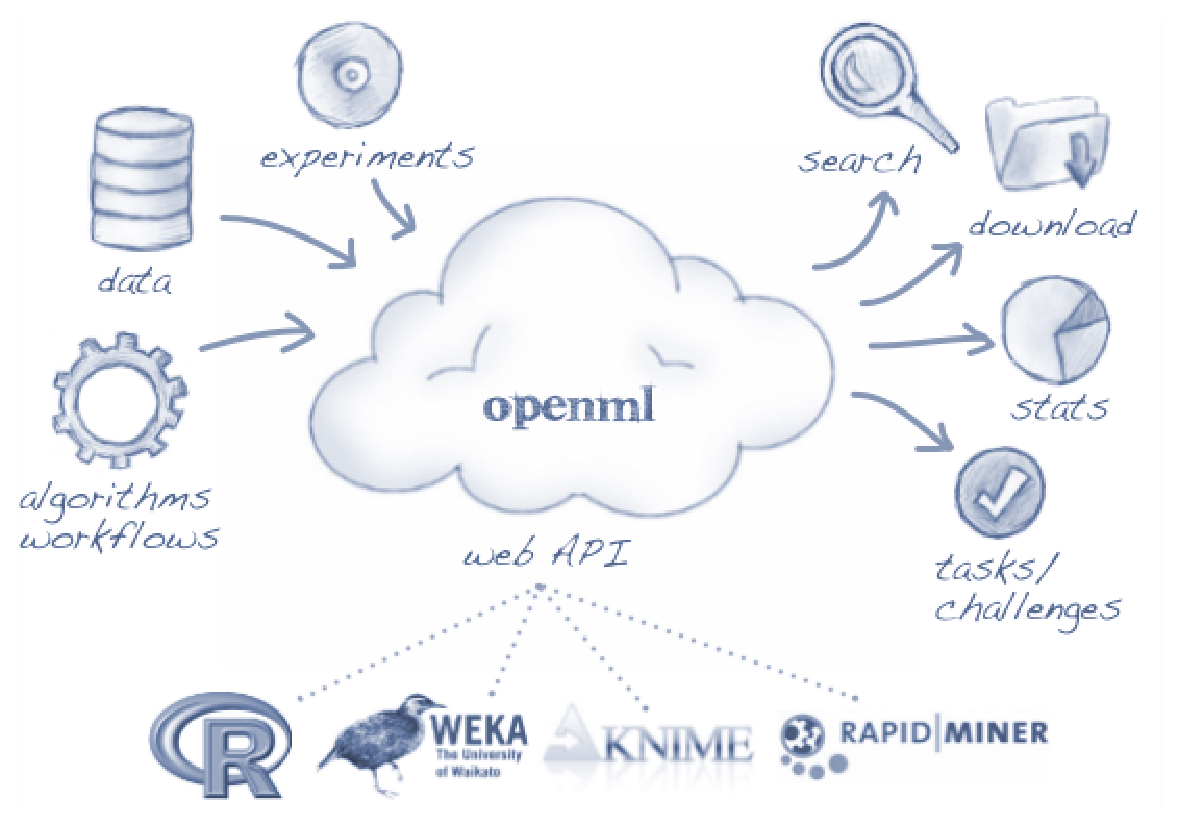
\includegraphics[width=.78\textwidth]{eps/openmldiagram.eps}
	\caption{Components of OpenML.}
	\label{fig:openmlOverview}
\end{figure}

The key components of OpenML are shown in Figure~\ref{fig:openmlOverview}. Central are the OpenML API and database, which contains all details and meta-data about all shared datasets, implementations and experiments. New content can be sent to OpenML by means of a RESTful API. This API is also being integrated into a number of popular data mining and machine learning tools, i.e., Weka, R, KNIME and RapidMiner, so that content can be shared automatically. OpenML also provides various search interfaces, so that these entities can later be retrieved, e.g., through a web interface, textual search engine or SQL interface. The latter enables users to directly query the database by means of SQL statements. 

In Section~\ref{sec:Related} an overview of related work is provided. In Section~\ref{sec:Tasks}, we discuss how experiments are defined in OpenML. Section~\ref{sec:Database} provides an overview of the most important concepts in the database. In Section~\ref{sec:API} we describe the web API, allowing integration into various tools. Section~\ref{sec:Sharing} describes how we support the sharing of experiments, and how it is being integrated into RapidMiner. Section~\ref{sec:Searching} details the search interfaces of OpenML, and Section~\ref{sec:Summary} concludes. 

\section{Related Work}
\label{sec:Related}
OpenML builds upon previous work on experiment databases~\cite{Vanschoren2012}, which introduced the idea of sharing machine learning experiments in databases for in-depth analysis of learning algorithms. The most notable enhancement of OpenML is the introduction of a web API to allow integration with various machine learning tools, and a more clear definition of experiments through \emph{tasks} (see Section~\ref{sec:Tasks}).

Kaggle\footnote{\texttt{http://www.kaggle.com/}} is a platform which hosts machine learning challenges. In some sense, these challenges are similar to OpenML tasks: users are provided with data and instructions, and challenged to build a predictive model on this. However, as Kaggle is a competition platform, it does not support collaboration: people are not allowed to see each other's algorithms or results. OpenML, however, is an open science platform, allowing researchers complete insight into each other's work. 

There also exist several platforms for sharing algorithms, workflows and datasets, such as myExperiment~\cite{Roure2009,Goble2010} and MLData.\footnote{\texttt{http://www.mldata.org/}} However, these platforms were not designed to collect and organise large amounts of experimental results over many algorithms and datasets, nor allow such detailed analysis of learning algorithms and workflows afterwards. On the other hand, we do aim to fully integrate these platforms with OpenML, so that datasets and algorithms can be easily transferred between them. 

Finally, MLComp\footnote{\texttt{http://www.mlcomp.org/}} is a service that offers to run your algorithms on a range of datasets (or vice versa) on their servers. This has the great benefit that runtimes can be compared more easily. This is not strictly possible in OpenML, because experiments are typically run on the user's machines. However, OpenML does allow you to rerun the exact same experiments on different hardware, which is necessary anyway since hardware will change over time. Moreover, researchers do not need to adapt the way they do their research: 
they can run their algorithms in their own environments. OpenML also allows users to define different types of experiments beyond the traditional benchmarking runs, and allows more flexible search and query capabilities beyond direct algorithm comparisons.

\section{Tasks}
\label{sec:Tasks}
In order to make experiments from different researchers comparable, OpenML fully defines experiments in \emph{tasks}. A task is a well-defined problem to be solved by a machine learning algorithm or workflow. For each task, the inputs are provided and the expected output is defined.  An attempt to solve a task is called a~\emph{run}. Currently, tasks of the type \emph{Supervised Classification} and \emph{Supervised Regression} are supported, but OpenML is designed in such a way that it can be extended with other task types. A typical task would be: \emph{Predict target variable X on dataset Y with a maximized score for evaluation metric Z}. Usually, when a user wants to submit new results to the server, he searches for appropriate tasks, and runs his algorithm on these. The results from these runs will be uploaded to the server, along with information about the algorithm, its version and the parameter settings. This process is explained in detail in Section~\ref{sec:API}.

\begin{figure}[ht!]
	\lstinputlisting[language=XML]{misc/task.xml}
	\caption{XML representation of a task.}
	\label{fig:taskxml}
\end{figure} 

Figure~\ref{fig:taskxml} shows an example of a Supervised Classification task definition. It provides all information necessary for executing it, such as a URL to download the input dataset and an \emph{estimation procedure}. The estimation procedure describes how the algorithms that are run on this task are being evaluated, e.g., using cross validation, a holdout set or leave-one-out. For every run performed on a certain task, this is done using the same data splits. An ARFF file containing these splits is provided. Also, a set of \emph{evaluation measures} to optimise on is provided. An ARFF file containing the predictions (and confidences per class) is expected as the result.

\section{Database}
\label{sec:Database}
One of the key aspects of OpenML is the central database, containing details about all experiments. A partial schema of the database is provided in Figure~\ref{fig:dbschema}. 
In the database schema, the concept of \emph{inheritance} is used: some tables shown do not exist, but describe what fields should be contained by tables inheriting from them, i.e., \texttt{data} and \texttt{setup}. We call these tables \emph{interface tables}. Also, all tables inheriting from the same interface table share a primary key. 

\begin{figure}[ht!]
	\centering
	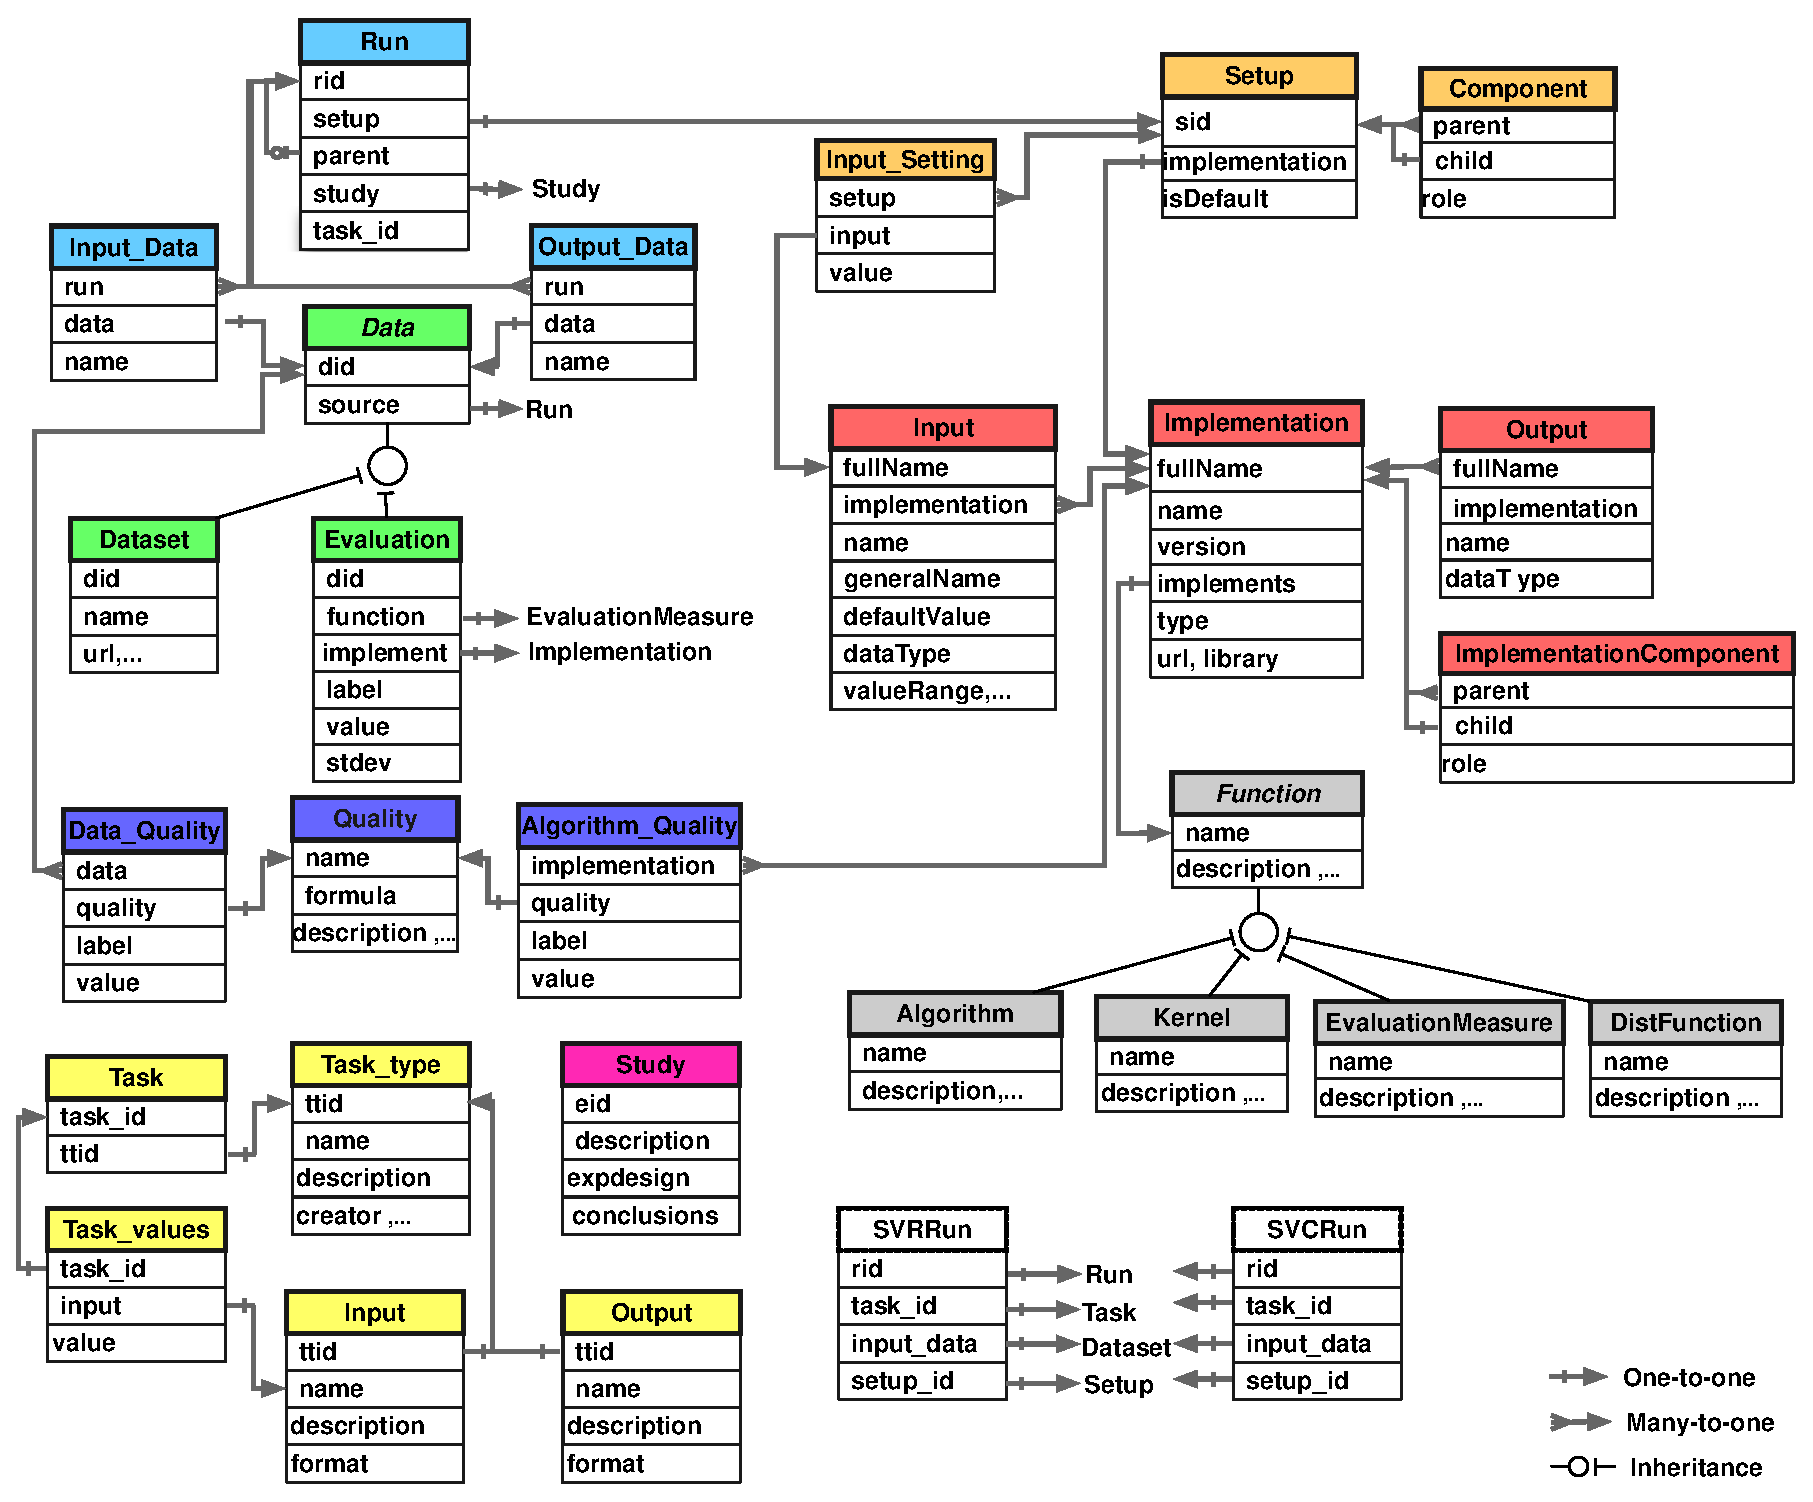
\includegraphics[width=\textwidth]{eps/dbschema.eps}
	\caption{Database schema.}
	\label{fig:dbschema}
\end{figure} 

OpenML considers algorithms as conceptual entities, an algorithm itself can not be used to execute a task. Instead, an algorithm can be implemented, resulting in an \emph{implementation}. In this way we also support versioning. For example, when an implementation containing a bug is used, this will potentially yield suboptimal results. This changes whenever a new version is released. Thus, we use the table \texttt{implementation}, where the primary key is \texttt{fullName}, an aggregation of its name (field: \texttt{implementation}) and its version (field: \texttt{version}). More specifically, an implementation can typically be run with different parameter settings. The \texttt{setup} table contains, for each implementation, which parameter values where used in a specific run. The table \texttt{input} contains for each implementation all parameters and their default values. The table \texttt{input\_setting} contains for every setup the values of the parameters. 

The tables \texttt{dataset} and \texttt{evaluation} both contain data, which can serve as input or output of a \texttt{run}. These are linked together by the linking tables \texttt{input\_data} and \texttt{output\_data}. 
Entries in the \texttt{dataset} table can be either user-submitted datasets or files containing the result of a run, such as predictions. For each evaluation measure performed, an entry is stored in the \texttt{evaluation} table. 
Querying all experiments of a specific type of task is easiest if the inputs and outputs of that task types are combined in a single table. For this reason, the views \texttt{SVCRun} and \texttt{SVRRun} have been introduced for Supervised Classification tasks and Supervised Regression tasks, respectively. These are materialized views containing all inputs, outputs and results of such an experiment. 

For each implementation and dataset, a number of meta-features~\cite{Peng2002} are obtained and stored in the \texttt{data\_quality} and \texttt{algorithm\_quality} table, respectively. These meta-features are called \emph{qualities}. A list of all qualities can be found in their corresponding tables. 

\section{RESTful API}
\label{sec:API}
In order to enable the sharing of experiments, a web API\footnote{Full documentation of the API can be found at \texttt{http://www.openml.org/api/}} has been developed. The API contains functions that facilitate downloading datasets, tasks and implementations. Furthermore, it enables the uploading of datasets, implementations and runs. The API also contains functions that list evaluation measures, licence data and evaluation methods. We will briefly explain the most important features. 

\begin{figure}[ht!]
	\centering
	\begin{subfigure}{.48\textwidth}
		\centering
		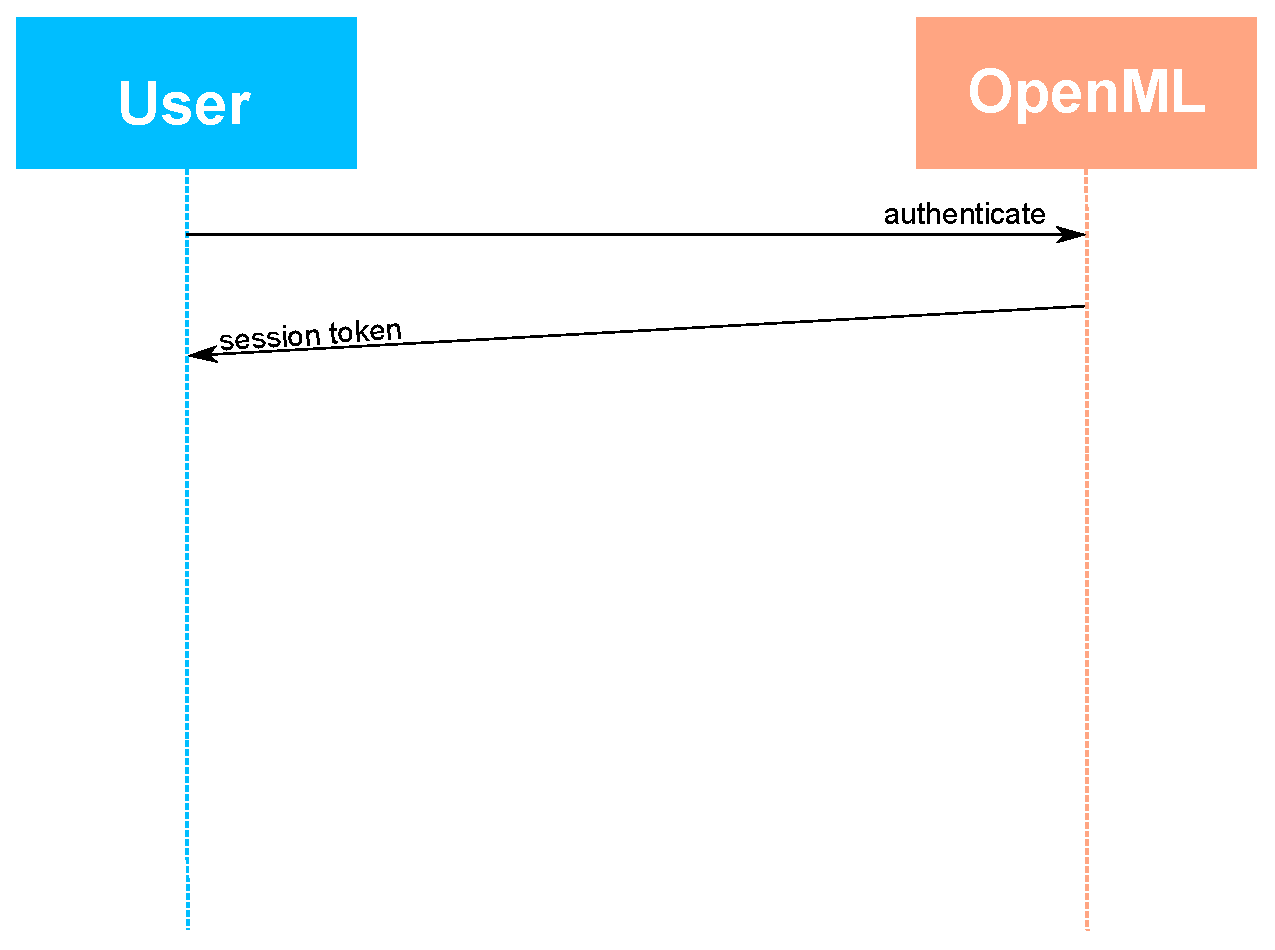
\includegraphics[width=\textwidth]{eps/api_authenticate.eps}
		\caption{Authenticate}
		\label{fig:api_authenticate}
	\end{subfigure}
	\hspace{2 mm}
	\begin{subfigure}{.48\textwidth}
		\centering
		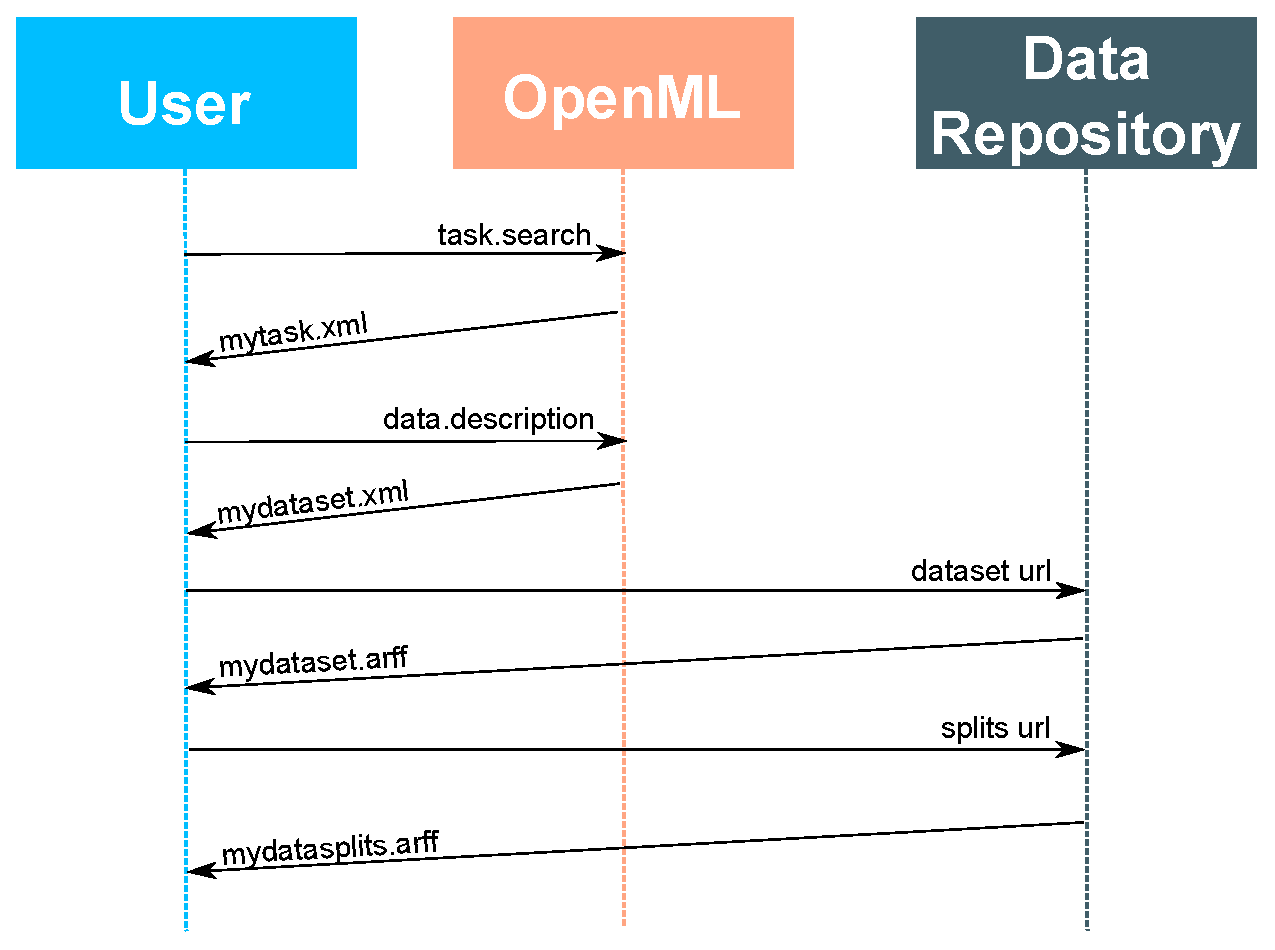
\includegraphics[width=\textwidth]{eps/api_task.eps}
		\caption{Download task}
		\label{fig:api_task}
	\end{subfigure}
	\begin{subfigure}{.48\textwidth}
		\centering
		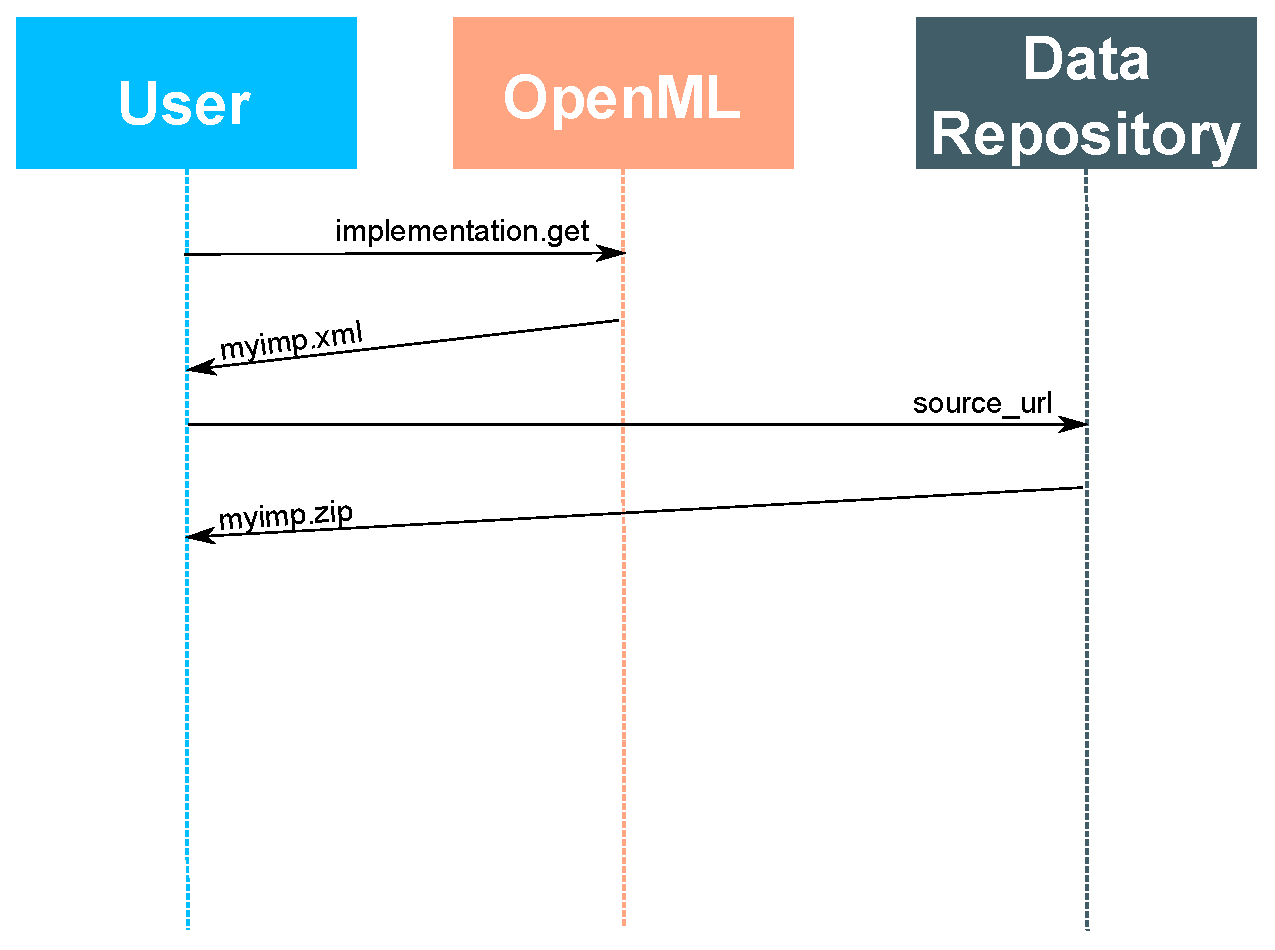
\includegraphics[width=\textwidth]{eps/api_implementationget.eps}
		\caption{Download implementation}
		\label{fig:api_implementation}
	\end{subfigure}
	\hspace{2 mm}
	\begin{subfigure}{.48\textwidth}
		\centering
		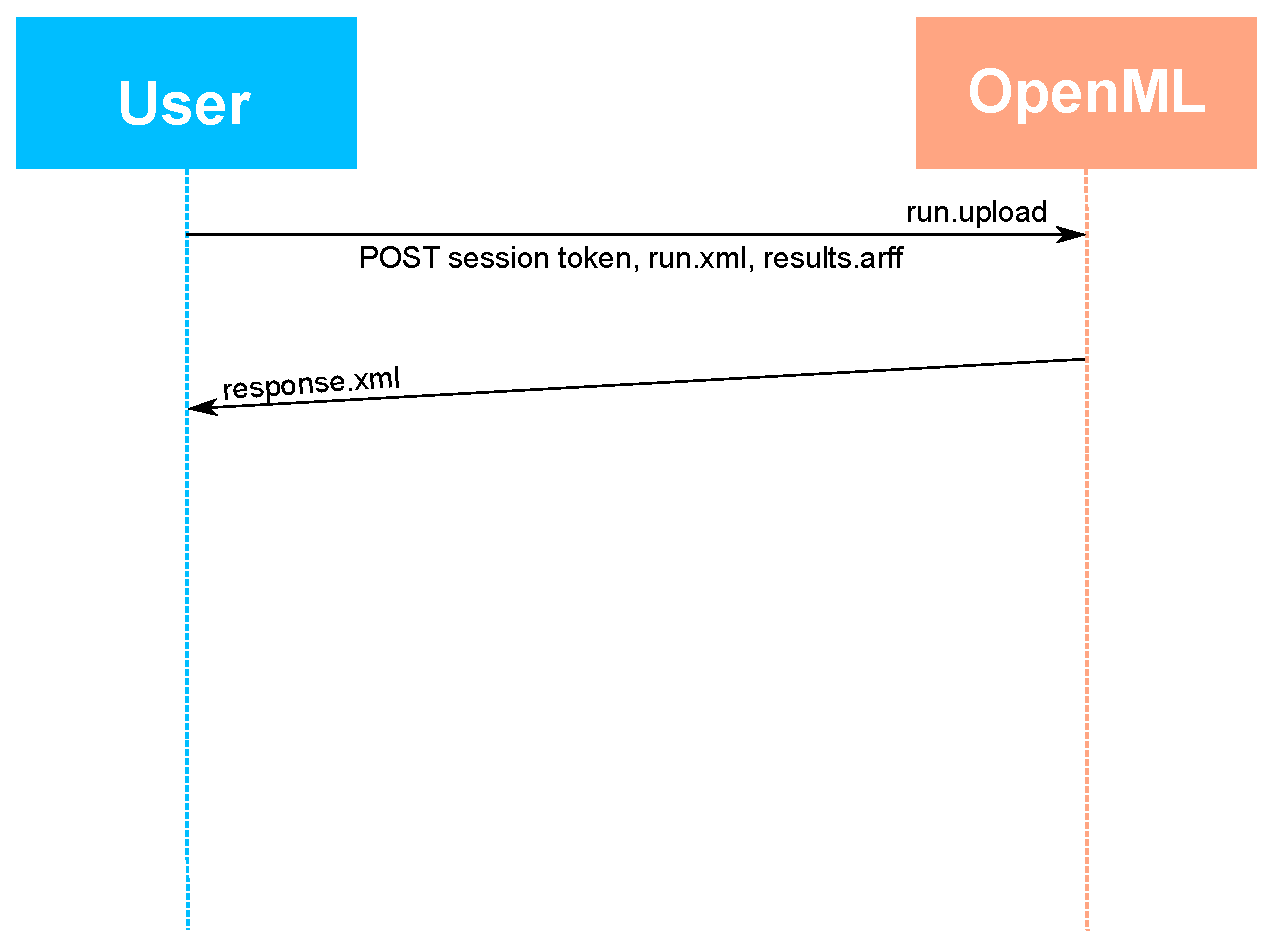
\includegraphics[width=\textwidth]{eps/api_run.eps}
		\caption{Upload run}
		\label{fig:api_run}
	\end{subfigure}
	\caption{Use case diagrams of the API.}
	\label{fig:apidiagrams}
\end{figure} 

Functions that involve the uploading of content require the user to provide a \emph{session hash}. A session hash is a unique string which is used to authenticate the user. It is valid for a limited amount of time. Users can obtain a session hash by invoking the function \texttt{openml.authenticate} (see also Figure~\ref{fig:api_authenticate}). Inputs for this function are the username and an MD5 hash of the passwords. 

Tasks can be obtained by invoking the function \texttt{openml.task.search}. An XML file, similar to the XML file shown in Figure~\ref{fig:taskxml}, is returned. The source data described is an ID referring to a dataset. In order to obtain information concerning this dataset, including a download URL, users should perform an additional call to \texttt{openml.data.description}. The dataset can reside in any data repository, including a user's personal webpage. Figure~\ref{fig:api_task} details on how the content of a task is obtained.  

Datasets and implementations can be obtained using the API. Both are referred to with an ID. By invoking the functions \texttt{openml.data.description} and \texttt{openml.implementation.get} with this ID as parameter, users obtain an XML file describing the dataset or implementation. Figure~\ref{fig:api_implementation} shows how to download an implementation. Datasets can be obtained in a similar way. 

Runs can be submitted by invoking the function \texttt{openml.run.upload}. Figure~\ref{fig:api_run} outlines how this works. The user provides an XML file describing which implementation was used, and what the parameter settings were. The implementation that was used should already be registered on OpenML. Furthermore, all output of the run must be submitted. For the supervised classification and regression tasks, this will include a file with predictions, which will be evaluated on the server and stored in the database. The server will return an ID referring to the record in the database. Uploading datasets and implementations happens in a similar way. For this the functions \texttt{openml.data.upload} and \texttt{openml.implementation.upload} are used, respectively. 

A list of all evaluation measures for usage in tasks can be obtained by invoking \texttt{openml.evaluation.measures}. 

\section{Sharing Experiments}
\label{sec:Sharing}
To facilitate the sharing of experiments, plugins are being developed for popular data mining and machine learning tools, including RapidMiner. The RapidMiner plugin can be downloaded from the OpenML website. It introduces three new operators. 

The \emph{Read OpenML Task} operator handles the downloading of tasks. When presented with a task id, it automatically downloads this task and all associated content, i.e., the input dataset and the data splits. Every entity downloaded from OpenML is cached on the user's local disk. The operator composes the various training and test sets, and marks attributes with certain roles as such, e.g. the target attribute or a row id. 

The resulting training and test set will be sent to the \emph{OpenML Prediction} operator. For each training set submitted to this operator, a predictive model is built, which generates predictions for all instances in the test set. These predictions will be sent to the \emph{Share on OpenML} operator, which is responsible for submitting the results to OpenML. First, it checks whether the implementation already exists, and if not, it will be registered. After that, all parameter values are tracked. Finally, an XML file describing the run and an ARFF file containing the predictions will be sent to OpenML.

\begin{figure}
	\begin{subfigure}{\textwidth}
		\centering
		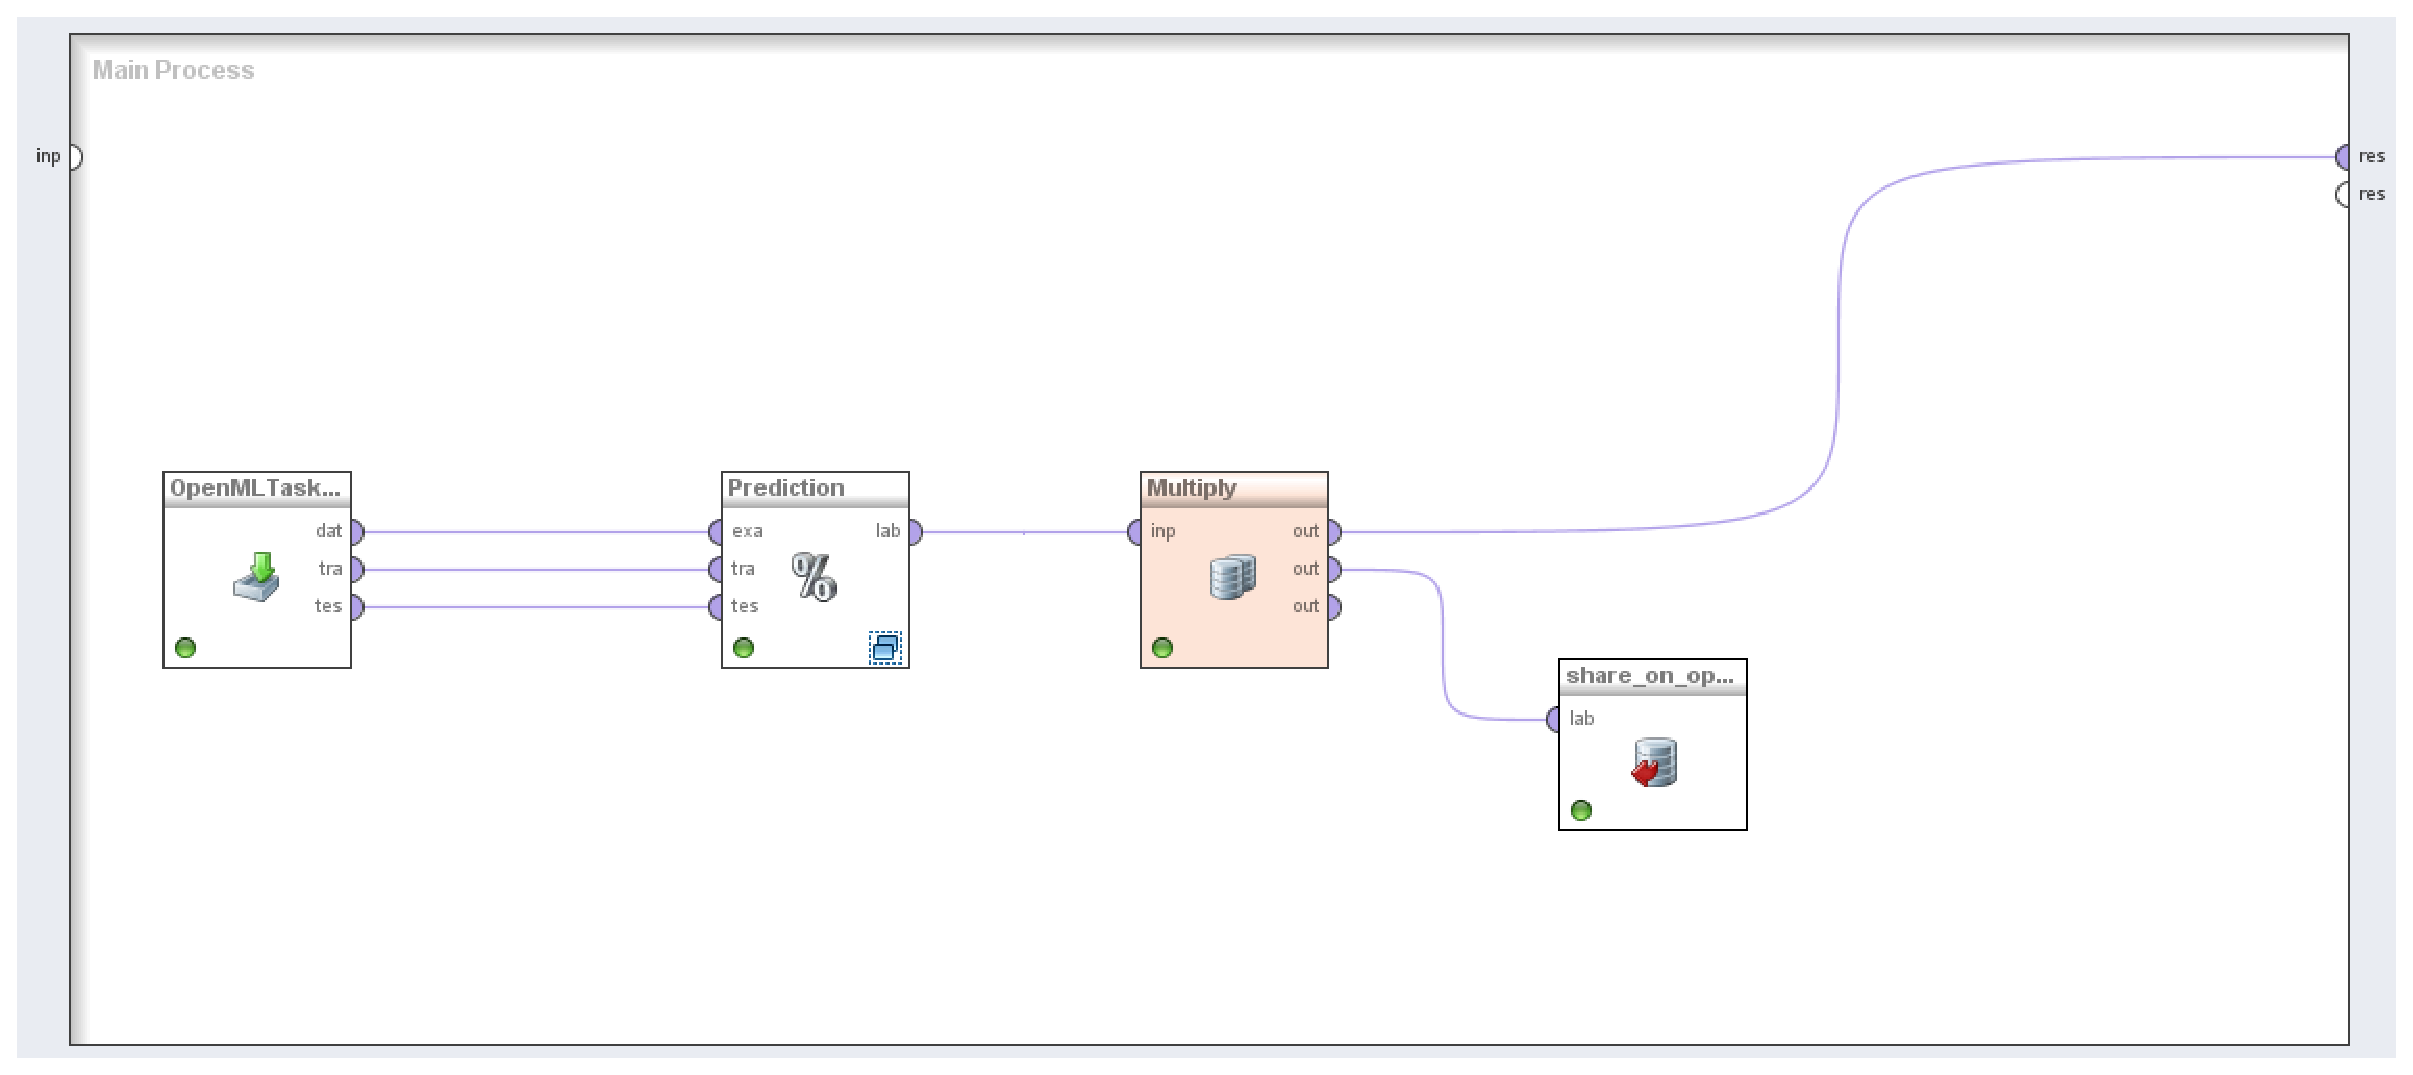
\includegraphics[width=\textwidth]{eps/RapidMinerWorkflow.eps}
		\caption{Global Workflow.}
		\label{fig:globalWorkflow}
	\end{subfigure}
	\begin{subfigure}{\textwidth}
		\centering
		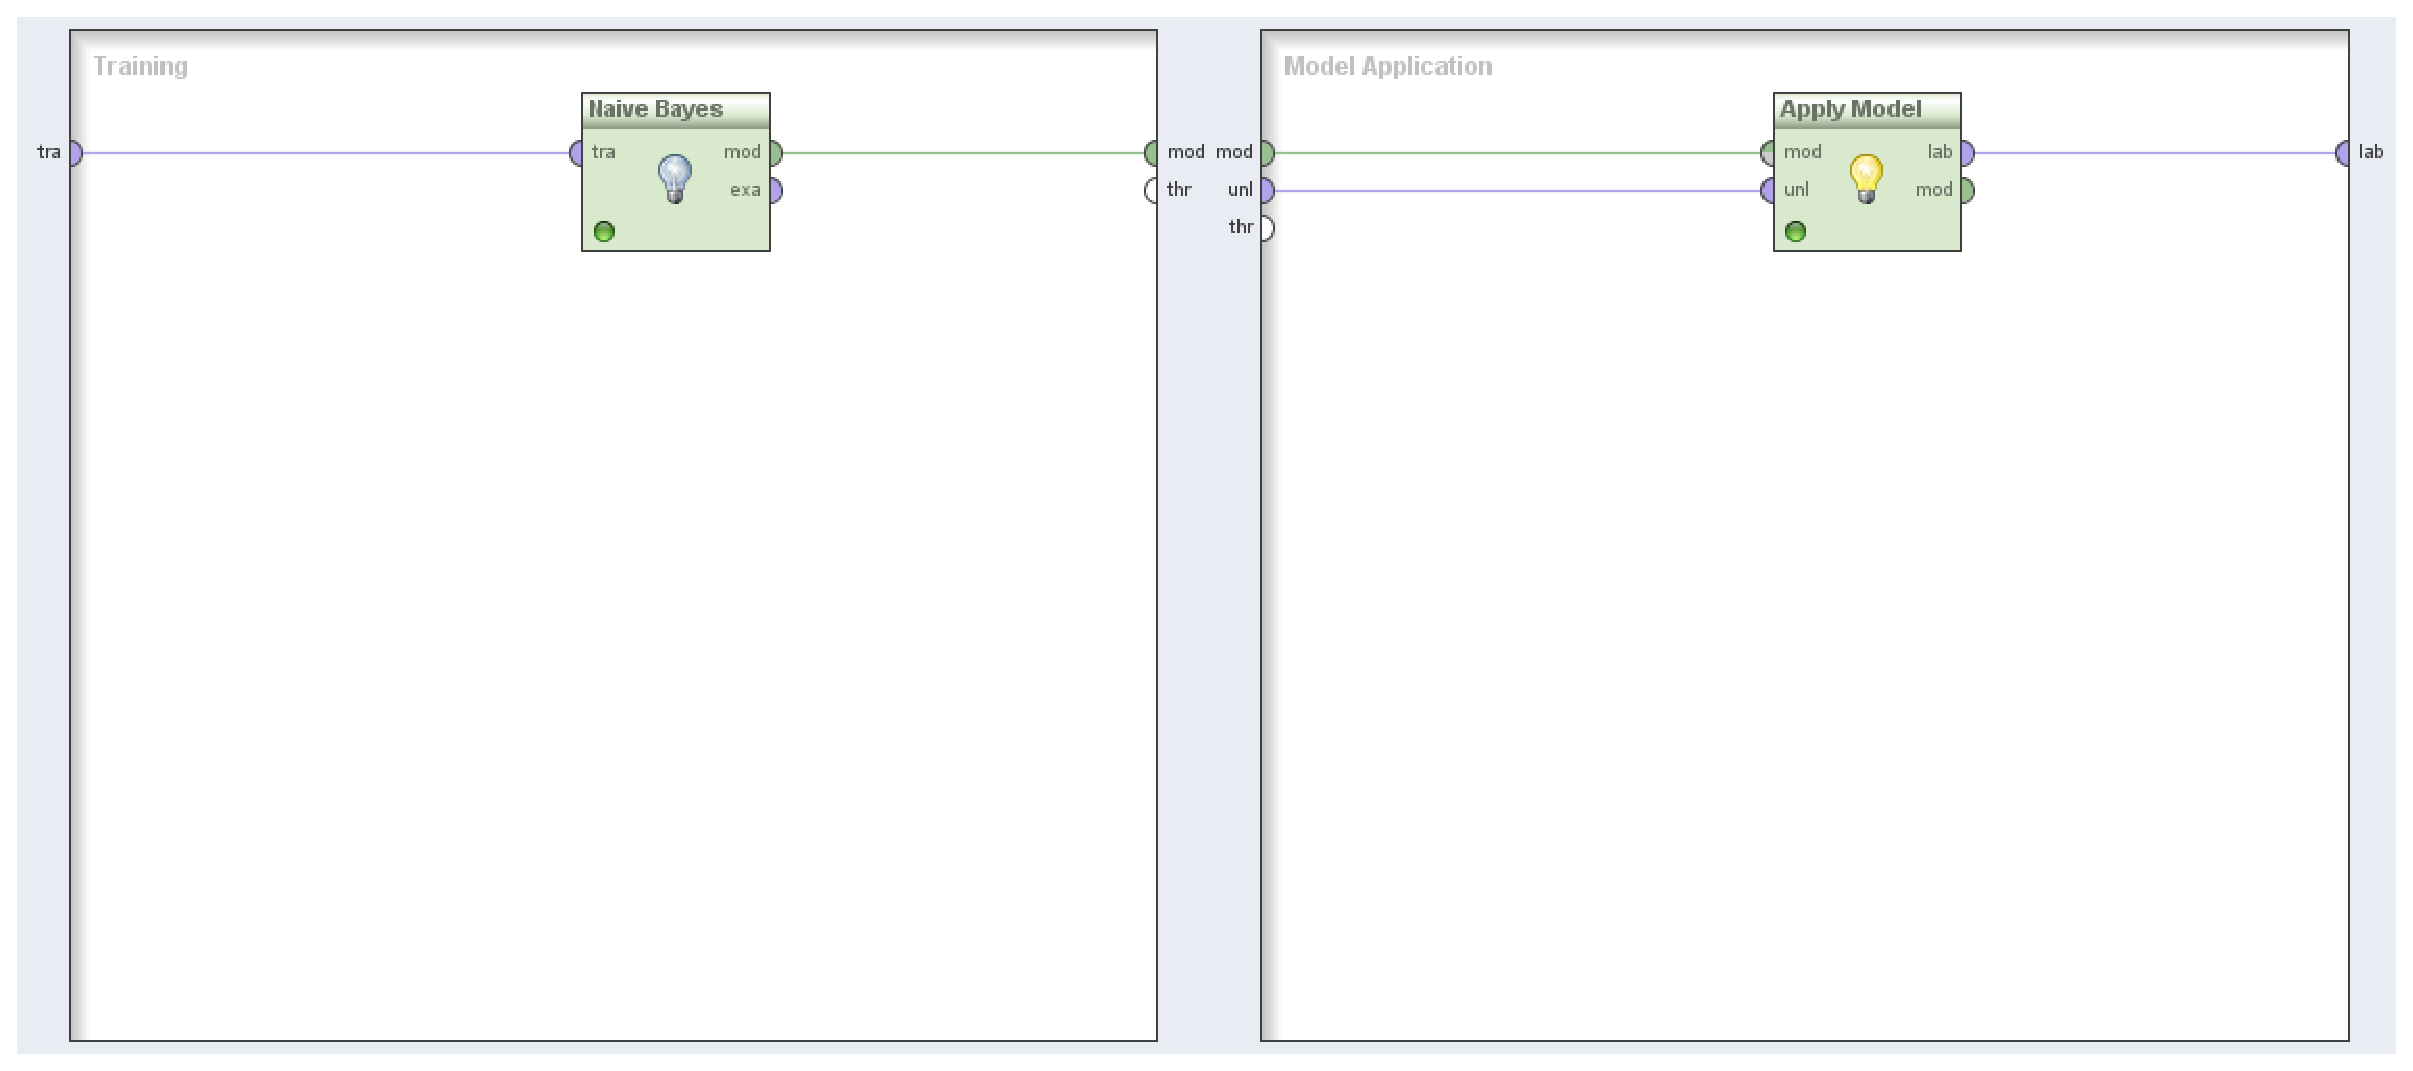
\includegraphics[width=\textwidth]{eps/RapidMinerPrediction.eps}
		\caption{Sub workflow of the OpenML Prediction operator.}
		\label{fig:subWorkflow}
	\end{subfigure}
	\caption{Workflow which downloads an OpenML task, and sends back the results.}
	\label{fig:exampleWorkflow}
\end{figure}

Figure~\ref{fig:exampleWorkflow} contains a workflow which uses these operators. This workflow can also be downloaded from the website. Before it can be run, a local directory for caching the downloaded data is required. This can be done in the Preferences menu, under the OpenML tab. When this is set, a workflow containing the OpenML operators can be created. A global outline is shown in Figure~\ref{fig:globalWorkflow}. The operators are connected to each other in a straightforward way. We used a \emph{multiply} operator to split the outcome of the Prediction operator to both the general output and the Share on OpenML operator. Note that if the user does not want to share his results on line, he can simply omit the Share on OpenML operator. 

By clicking on the OpenML Prediction operator, a screen similar to Figure~\ref{fig:subWorkflow} is shown. This is where subworkflows can be created, to handle both the training and the test data. As for the subworkflow that handles the training data, make sure that at least a model is created, e.g., by including a \emph{Naive Bayes} operator. For the Model application part it typically suffices to insert an \emph{Apply Model} operator. 
Finally, as parameter of the Read OpenML Task operator, a task id should be provided. These can be searched from the OpenML website. 

\section{Searching OpenML}
\label{sec:Searching}
All experiments in the database are openly available to everyone. Several ways of searching through these experiments are provided.\footnote{\texttt{http://www.openml.org/search/}} The most notable ways of searching through OpenML are textual search, the ``search runs'' interface and the SQL interface.

All implementations, datasets and evaluation metrics submitted to OpenML are required to include meta-data, such as a name, textual description, licence data and in the case of implementations, installation notes and dependencies. These textual descriptions are indexed by a search engine running on the website, so that implementations and datasets can be searched through keywords. 

The ``search runs'' is a wizard interface specialized in benchmark queries. It can be found under the `Advanced' tab of the search page. The user is presented with a form where he specifies which datasets (or collections of datasets) and implementations he is interested in. Furthermore, he specifies on which evaluation measure the benchmark should be performed. Typical questions that can be answered with this interface are ``what implementation performs best on dataset X'', ``compare several implementations on all datasets'', ``show the effect of data property DP on the optimal value of parameter P'' and ``how influence parameter settings the performance of implementation X''.

\begin{figure}[ht!]
	\centering
	\begin{subfigure}{\textwidth}
		\lstinputlisting[language=SQL,numbers=none,breaklines=true]{misc/learningcurve.sql}
		\caption{SQL statement}
		\label{fig:comparesqlCode}
	\end{subfigure}
	\begin{subfigure}{.75\textwidth}
		\centering
		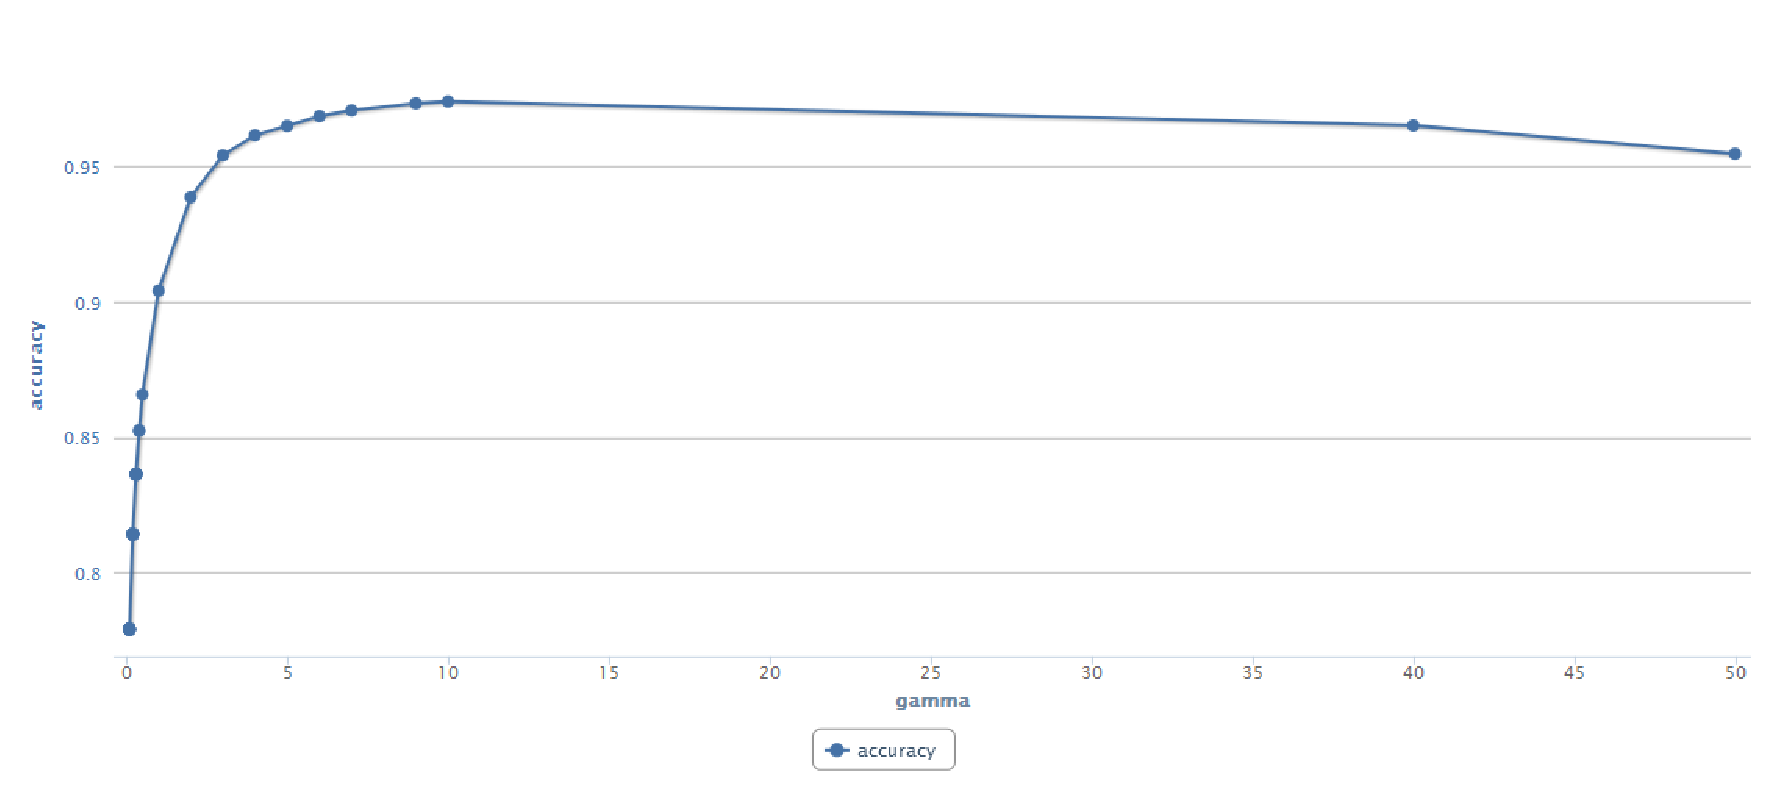
\includegraphics[width=\textwidth]{eps/learningcurve.eps}
		\caption{Line plot of the result}
		\label{fig:comparesqlLineplot}
	\end{subfigure}
	\caption{Studying the effect of a parameter.}
	\label{fig:comparesql}
\end{figure} 

The most flexible way of searching through OpenML is querying the database directly by means of SQL statements. With some knowledge of the database (see Section~\ref{sec:Database}) complex queries can be executed in any way the user wants it. Under the `Advanced' tab of the search page some queries are provided. The user can also inspect the SQL code of these queries, so these can be adapted to the user's specific needs. In Figure~\ref{fig:comparesql} an example of such a query is provided. It studies the effect of the gamma parameter of the Weka implementation of a Support Vector Machine, on the UCI letter dataset~\cite{frey1991}. 

The results of queries can be obtained in CSV and ARFF format. Furthermore, scatterplots and line plots (as shown in Figure~\ref{fig:comparesqlLineplot}) are provided. 

\section{Summary}
\label{sec:Summary}
OpenML aims to stimulate an open approach to machine learning research, by collecting results in a database. In order to provide an easy way of sharing these, plugins for various machine learning tools will be provided, including RapidMiner. Instead of running experiments over and over again, users can easily query the database and obtain the results on relevant research questions. 

Future work on OpenML includes the integration with other machine learning platforms, such as MLData and myExperiment. Also, the support for a broader range of task types, such as time series analyses, feature selection and graph mining, will be provided. Future work on the RapidMiner plugin includes a better integration with the various services of OpenML. Currently, the plugin is mainly focussed on downloading tasks and uploading results. Features like downloading workflows, uploading datasets and inspecting results could be valuable additions to the plugin. 

\subsubsection*{Acknowledgments}
This work is supported by grant 600.065.120.12N150 from the Dutch Fund for Scientific Research (NWO), and by the IST Programme of the European Community, under the Harvest Programme of the PASCAL2 Network of Excellence, IST-2007-216886.

\bibliographystyle{plain}
\bibliography{rcomm2013}

\end{document}
